\documentclass[10pt,a4paper]{article}
\usepackage[dutch]{babel}
\usepackage{hyperref}
\usepackage{a4wide}
\usepackage{graphicx}
\title{BYOD handout 2019}
\author{Erik Kooistra \& Sam van Kampen}

\AtEndDocument{\label{last_page}}
\begin{document}

\maketitle

\tableofcontents

\section{Introductie}

Op de wiki die speciaal is ingericht voor de ``Bring Your Own Device''
van de bachelors Informatica en Kunstmatige Intelligentie staan uitgebreide instructies
om jouw laptop dual-boot te maken. Een gedeelte van deze wiki staat in deze hand-out zodat
je geen extra computer nodig hebt om de wiki op te openen.
De wiki is terug te vinden op: \url{https://linux.datanose.nl}

Het installeren bestaat uit \ref*{last_page}  stappen die ieder een eigen hoofdstuk kennen.
Lees de teksten zeer zorgvuldig door en stel bij twijfel altijd vragen!

Je bent pas klaar als niet alleen jouw laptop, maar ook die van je medestudenten werken.
Mocht je geen USB-stick mee hebben genomen, dan kun je gebruik maken van een reserve-USB-stick.

\section{BitLocker}

Op sommige laptops, voornamelijk zakelijke laptops, kan het voorkomen dat BitLocker standaard
aanstaat. Als dat het geval is is het het makkelijkst om BitLocker eerst het uit te zetten voordat
je Ubuntu installeert. Als je wilt weten of BitLocker aanstaat en hoe je het kan uitzetten
of hoe je Ubuntu kan installeren met BitLocker aan, zie \url{https://linux.datanose.nl/index.php/BitLocker}.


\section{Fast Start-up uitschakelen}

Open het configuratiescherm, en selecteer in het menu de optie ``Power Options''. Voor visuele referentie zie \ref{img:fast}.
Links zie je dan een lijst aan opties staan,
selecteer daar de optie ``Choose what the power buttons do''.
Klik dan op ``Change settings that are currently unavailable'' (in het blauw).
Scroll naar beneden totdat je een lijstje met opties ziet,
en schakel dan ``Turn on fast start-up (recommended)'' uit.
Tenslotte klik je dan op ``Save Changes'' om het te bevestigen.

\begin{figure}[t]
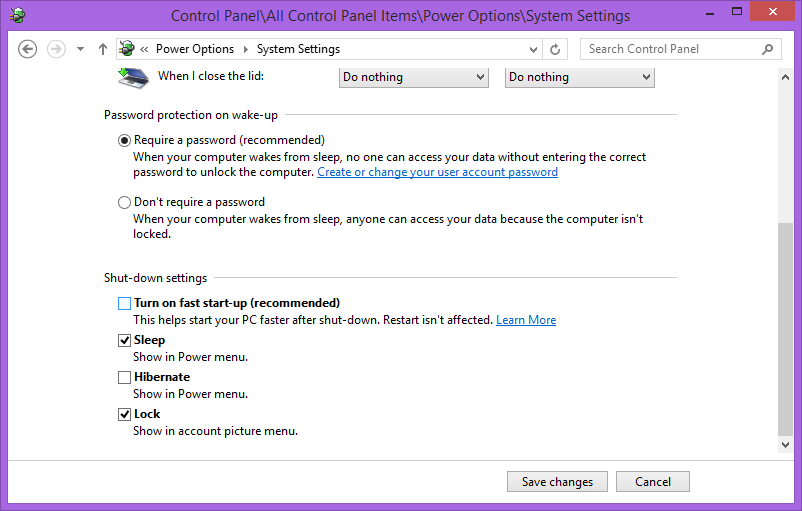
\includegraphics[width=0.9\textwidth]{fast-startup}
\caption{Fast startup control panel}
\label{img:fast}
\end{figure}

\section{Microsoft Secure Boot uitschakelen}

Ga naar het menu waar je de computer kan uitzetten, herstarten, etc.
Houd de Shift-toets ingedrukt terwijl je op de optie om te herstarten klikt.
Er verschijnt nu een menu met verschillende opties.
Selecteer de ``Troubleshoot''-optie.
Daarna verschijnt er weer een menu, selecteer ``Advanced Settings''.
Tenslotte verschijnt er nog een menu, selecteer ``UEFI Firmware Settings''.
De computer zal dan herstarten en opstarten in het configuratiescherm van de UEFI-implementatie zelf.
Mocht het niet mogelijk zijn om op deze manier in het configuratiescherm van UEFI te geraken,
dan is het ook mogelijk dat er een specifieke toetsencombinatie moet ingedrukt worden
tijdens het opstarten van de computer. Als dat het geval is, raadpleeg dan Google om achter deze
toetsencombinatie van je laptop te komen.
Als alles in orde is, dan kan je in het configuratiescherm van UEFI navigeren
naar de ``Secure Boot''-optie, en deze uitzetten. Soms is het niet mogelijk om deze optie
uit te schakelen als er geen administrator-wachtwoord ingesteld is in de UEFI. Als dit het geval is, stel een wachtwoord in. Houd deze makkelijk, want als je deze vergeten bent kan je niet meer je UEFI-instellingen in.

\section{Voorbereiden van de USB-stick}

Deze stappen heb je misschien thuis al uitgevoerd -- als je dit nog niet thuis gedaan hebt, kan je de volgende stappen volgen.
Zorg allereerst dat je een lege USB-stick van minstens 2 GiB hebt en
voer vervolgens de volgende stappen uit:
\begin{itemize}
\item Download het ISO-bestand van de 64-bit versie van Ubuntu 18.04.3 via de \url{https://ubuntu.com} website.
\item Download het programma \verb|usbwriter| (\url{http://sourceforge.net/projects/usbwriter/}
\item Gebruik het programma om de ISO als bronbestand te schrijven naar de USB-stick.
\end{itemize}


\section{Installatie}

Nu je de Ubuntu-installatie op een USB-stick hebt gezet,
is het tijd om de installatie vanaf de USB-stick voort te zetten.

\subsection{Opstarten vanaf de USB-stick}
Sluit de USB-stick aan op de computer, en start de computer op.
Als het goed is, start de computer op vanaf de USB-stick.
Mocht de USB-stick niet opstarten, dan moet de USB-stick opgestart
worden via het UEFI- of BIOS-configuratiescherm.
De makkelijkste manier om dat configuratiescherm op te starten is door
Windows op te starten, en naar het menu te gaan waar je de computer kan uitzetten, herstarten, etc.
Houd de Shift-toets ingedrukt terwijl je aldaar op de optie om te herstarten klikt.
Er verschijnt nu een menu met verschillende opties. Selecteer de ``Troubleshoot'' optie.
In dit menu is het mogelijk om met de optie ``Use a device'' te booten vanaf de USB-stick.

Mocht het niet mogelijk zijn om op deze manier te booten, dan is het ook mogelijk dat er een
specifieke toetsencombinatie moet ingedrukt worden tijdens het opstarten van de computer.
Als dat het geval is, raadpleeg dan Google om achter deze toetsencombinatie van je laptop te komen.
Als alles in orde is, dan kan je in het configuratiescherm navigeren naar een optie
om vanaf een USB-apparaat op te starten.
\subsection{Het Ubuntu-opstartkeuzemenu}
Zodra je laptop is opgestart vanaf de USB-stick krijg je een keuzemenu te zien.
Selecteer hier de optie ``Try Ubuntu'' of ``Try Ubuntu without installing''.
Daarna zal er een liveomgeving van Ubuntu opgestart worden,
waar je Ubuntu in principe kunt uitproberen. Als op dit moment Ubuntu niet opstart of het scherm
zwart blijft, kan dit liggen aan de videokaart die in je laptop zit. Je kan dit oplossen door tijdens
het opstarten wanneer je ``Try Ubuntu without installing'' kan kiezen, op ``e'' te drukken en
aan de regel die met \texttt{linux} begint \texttt{nomodeset} toe te voegen. en vervolgens op ``F10'' te
drukken.

\subsection{De Installatiewizard}
Nadat Ubuntu opgestart is kun je de installatieprocedure starten.
Maak verbinding met Eduroam (zie stap 7), en klik op ``Install Ubuntu 18.04 LTS''
om de installatiewizard op te starten. Als je onder Linux geen werkende WiFi hebt, start
dan de installatie zonder te verbinden met het internet, als de installatie klaar is steek dan
je hand dan gaan we daarna de WiFi-stuurprogramma's installeren.
Mochten de instructies op die pagina niet werken, stel dan een vraag.


\begin{figure}[t]
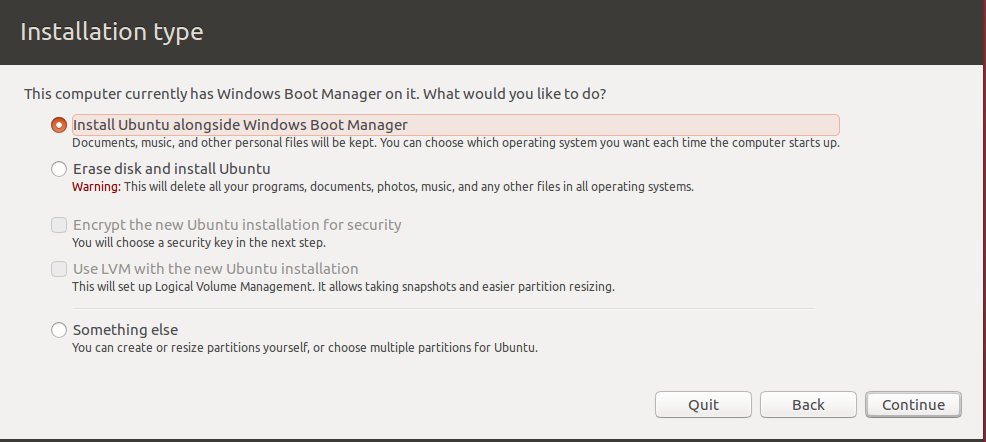
\includegraphics[width=0.9\textwidth]{install_type}
\caption{Installatie-opties}
\label{img:install}
\end{figure}

Als de installatiewizard is opgestart dan zal als eerste een taalkeuzemenu verschijnen.
Hiermee wordt de taal van het besturingssysteem ingesteld dat we gaan installeren.
Hier adviseren we ook om Engels te kiezen, omdat het dan
makkelijker is om documentatie raad te plegen, hulp te vragen, etc.

Het scherm daarna zal je vragen updates te downloaden tijdens de
installatie en software van derden te installeren. Vink beide opties aan.

In het scherm daarna zal je gevraagd worden hoe je Ubuntu precies wilt installeren.
Selecteer hier de optie ``Install Ubuntu alongside Windows Boot Manager'', zoals te zien in \ref{img:install}
Mocht dit niet verschijnen, vraag dan een van de begeleiders om hulp. % TODO ssd raid magic

\subsection{Linux kan de harde schijf niet vinden}

Als Linux de harde schijf niet ziet kan dit aan Intel RST liggen. Dit kan makkelijk opgelost worden
door de volgende stappen uit te voeren.
\begin{itemize}
     \item Start Windows op en open een commandovenster als administrator
     \item Voer \verb|bcdedit /set {current} safeboot minimal| uit
     \item Reboot en verander de SATA mode of soms de RST mode in de UEFI naar AHCI
     \item Boot Windows weer, start weer een commandovenster op als administrator en voer het volgende uit: \verb|bcdedit /deletevalue {current} safeboot|
     \item Nu zou de Ubuntu-installatie de disk wel moeten herkennen.
\end{itemize}
In het scherm erna kun je kiezen op welke harde schijf je
Linux Ubuntu gaat installeren, en hoeveel ruimte je wilt toewijzen aan beide besturingssystemen. Als je een SSD en een HDD in je laptop hebt zitten is het aan te raden om Linux op de SSD te zetten.
De installatiewizard zal je dan vragen of je zeker weet dat je wilt doen, omdat de bewerkingen die gedaan zullen worden niet ongedaan gemaakt kunnen worden.
Bevestig dat je dit wilt doen. Zorg ervoor dat je Ubuntu voldoende ruimte geeft, aangezien het een uitdaging is dit later te op te hogen.

Daarna zal er een scherm met een wereldkaart verschijnen, waarvan op basis van de keuze
van het land wat veronderstellingen gemaakt worden over de tijdzone,
de valuta, de decimale scheiding, etc.
In het scherm erna wordt gevraagd om de toetsenbordlayout in te stellen.
Als je Microsoft Windows gebruikt, raden we aan om ``English (US) intl.'' te kiezen. De versie met ``with dead keys'' erachter zorgt ervoor dat je speciale tekens als \'e kunt typen door achtereenvolgens het apostrofteken en de `e' te typen - kies deze layout als je dat gedrag wilt.
Als laatste wordt gevraagd om wat persoonlijke gegevens in te vullen zoals je volledige naam,
een gebruikersnaam, een wachtwoord, en een naam voor de computer.
Op Linux is de voorkeur om de gebruikersnaam en de computernaam in kleine letters te schrijven,
daarnaast is het aan te raden om een korte naam aan je computer te geven,
we raden een naam aan van maximaal
8 tekens.
Daarna zal de installatie beginnen.
Dit zal ongeveer een kwartier tot een uur duren afhankelijk van je laptop.
Als de installatie klaar is zal een dialoogvenster verschijnen met de vraag of je wilt herstarten.
Herstart het systeem.
Daarna zal er tijdens het herstarten een melding verschijnen dat je het installatiemedium moet
verwijderen.
Verwijder de USB-stick, en druk dan op de Enter-toets. Ubuntu zal dan opstarten.
Als je na het herstarten niet de optie krijgt om te kiezen tussen Ubuntu en Windows, stel dan een vraag.

\section{Eduroam-netwerk op Linux}

Het WiFi-netwerk van de UvA wordt aangeboden door eduroam.
Het netwerk maakt gebruik van WPA2 Enterprise. Klik rechtsboven in de system tray op het icoontje voor draadloze netwerk. Klik daarna op het WiFi-icoontje en selecteer Select Network, maak hier verbinding met het netwerk genaamd UvA.

\begin{description}
 \item[Authentication] TTLS of Tunneled TLS
 \item[Anonymous identity] anonymous@uva.nl
 \item[Domain] draadloos.uva.nl
 \item[CA certificate] Klik op 'Select from file...', typ dan \verb|/etc/ssl/certs/AddTrust_External_Root.pem| (als het goed is wordt de bestandsnaam automatisch afgemaakt).
 \item[Inner authentication] PAP
 \item[Username] studentnummer@uva.nl
 \item[Password] \textit{je wachtwoord}
\end{description}

\section{Pakketinstallatie}
Nadat Ubuntu is geïnstalleerd en je verbonden bent met het internet is het zaak enige pakketten te installeren die in de bachelor benodigd zijn.

Hiervoor hebben we een scriptje gebouwd dat je via de terminal moet uitvoeren. Open eerst een terminalvenster (Ctrl-Alt-T). Voer daar de volgende commando's in:\\

\noindent\verb|wget https://imgf.lt/install-extras.sh|\newline
\verb|chmod a+x install-extras.sh|\newline
\verb|sudo ./install-extras.sh|\newline

\textbf{N.B.} \texttt{sudo} vraagt om je wachtwoord, maar als je deze intikt verschijnen er geen tekens. Dat is de bedoeling - de tekens worden wel ingelezen, maar niet weergegeven.

Je wachtwoord ingevoerd hebbende krijg je een menu voorgeschoteld---nadat je je bachelor hebt gekozen in het menu worden de pakketten automatisch geïnstalleerd op je computer. Dit kan redelijk wat tijd kosten.

\end{document}
